\documentclass[conference]{IEEEtran}

\usepackage{cite}
\usepackage{amsmath,amssymb}
\usepackage{graphicx}
\usepackage{booktabs}
\usepackage{tikz}
\usepackage{xcolor}
\usepackage{hyperref}
\usepackage{pgfplots}
\pgfplotsset{compat=newest}

\hypersetup{
    colorlinks=true,
    linkcolor=blue,
    citecolor=blue,
    urlcolor=blue
}

\begin{document}

\title{Historical Case Study on Ti Silicide (TiSi\textsubscript{2}) \\ Reliability Issues in Mixed-Voltage CMOS Driver ICs}

\author{
\IEEEauthorblockN{Shinichi Samizo}
\IEEEauthorblockA{Independent Semiconductor Researcher\\
Project Design Hub, Samizo-AITL\\
\textit{Email:} \href{mailto:shin3t72@gmail.com}{shin3t72@gmail.com}\quad
\textit{GitHub:} \href{https://github.com/Samizo-AITL}{Samizo-AITL}}
}

\maketitle

\begin{abstract}
This paper analyzes a historical failure case at the 0.25~µm CMOS node related to Ti silicide (TiSi\textsubscript{2}) phase-transition instability. 
For active-matrix TFT (aTFT) LCD driver ICs that required mixed 3.3~V logic and $\sim$30~V high-voltage (HV) devices, manufacturers selected the 0.25~µm process because its LOCOS isolation safely supported HV co-integration. 
By contrast, the 0.18~µm STI-based node, although denser and yield-stable, posed edge-thinning risks for $\sim$30~V devices and required a new HV platform. 
Under this context, incomplete C49$\rightarrow$C54 transformation with boron absorption created localized high-resistance spots, directly reducing 1~Mbit SRAM yield. 
The study highlights how process optimization and empirical feedback cycles were indispensable when isolation technology and device requirements constrained node selection.
\end{abstract}

\section{Introduction}
In the late 1990s, LCD driver ICs for passive monochrome panels were commonly fabricated in 0.35~µm processes supporting 3.3~V logic and 40~V HV devices. 
With the transition to active-matrix TFT (aTFT) LCD panels in the early 2000s, driver ICs required higher-performance logic, embedded large SRAM macros, and continued HV integration around 30~V.  

Although the 0.18~µm CMOS process was already in mass production with small die size and stable yield, it relied on Shallow Trench Isolation (STI), where edge thinning introduced a reliability risk for $\sim$30~V devices. 
By contrast, the 0.25~µm process used Local Oxidation of Silicon (LOCOS), which had a proven track record for HV isolation. 
Therefore, manufacturers adopted the 0.25~µm LOCOS-based process for 3.3~V + 30~V LCD driver ICs, accepting area disadvantages to guarantee HV compatibility.

\section{Technical Background}
\subsection{Isolation Choice for HV Devices}
\begin{itemize}
    \item \textbf{0.25~µm LOCOS:} Mature, thick field oxide with well-established margins for $\sim$30~V HV device integration.
    \item \textbf{0.18~µm STI:} Provided density and yield benefits, but corner thinning at the trench edge raised leakage and breakdown concerns for HV devices, necessitating a new HV device platform.
\end{itemize}

\subsection{Ti Silicide Instability}
TiSi\textsubscript{2} was widely adopted for its low resistivity. However, it undergoes a phase transformation from metastable C49 to stable C54 during rapid thermal annealing (RTA).  
If the transformation remains incomplete, residual C49 grains act as high-resistance spots.  
Boron absorption from halo implants into Ti further aggravated resistivity variation.  
While these effects were tolerable in smaller SRAM macros (e.g., 500~kbit), they became fatal when scaled to 1~Mbit capacity.

\section{Failure Analysis}
\subsection{Observation: 1~Mbit SRAM}
In mass production, random single-bit failures appeared in the 1~Mbit SRAM macro. Since redundancy was not implemented in the embedded macro, even a single defective bit caused rejection of the entire device.

\subsection{Redundancy Limitation in Embedded Macros}
In stand-alone memory products, redundancy circuits are standard practice. Defective cells can be repaired during testing via laser trimming.  
In embedded memory macros, however, redundancy is generally excluded due to design complexity, timing, and area overhead.  
Additionally, LCD driver ICs were typically tested on mixed-signal/SoC testers, which lacked built-in support for redundancy repair.  
Therefore, redundancy was not adopted, and scaling to 1~Mbit carried critical reliability risk.

\subsection{Root Cause}
Failure localization confirmed that:
\begin{itemize}
    \item Boron from halo regions diffused into Ti during silicidation.
    \item Local B uptake inhibited C54 transformation, leaving high-resistance C49 spots.
    \item These spots manifested as random SRAM bit failures.
\end{itemize}

\subsection{Review Limitation}
Earlier 500~kbit SRAM macro products had not shown this issue. Based on those precedents, engineers assumed that scaling to 1~Mbit would be safe.  
Consequently, the failure mode was not identified during the initial development review stage, demonstrating the limitation of relying on past yield experience without revalidation.

\section{Countermeasures}
\subsection{Provisional Measures}
Etch profiles were tuned to slightly undercut sidewalls.  
This structural modification increased the physical separation between halo implant regions and the silicide formation area, reducing the probability of boron diffusion into Ti.  
As a result, localized inhibition of C54 transformation was temporarily suppressed, leading to short-term yield improvement.  
However, this countermeasure relied on process-window tuning and could not guarantee robustness across all wafer lots.

\subsection{Permanent Measures}
RTA conditions were optimized to promote complete transformation to the stable C54 phase.  
By carefully controlling temperature ramp rate and soak time, the process minimized residual C49 grains.  
This measure stabilized silicide resistivity, but at the cost of altering transistor series resistance and junction leakage, requiring re-characterization of device models and circuit timing libraries.  
Thus, the permanent solution involved a trade-off between silicide stability and overall device parameter shifts.

\section{Yield Sensitivity Model}
The yield impact of redundancy can be approximated by a Poisson model:
\[
Y_k = e^{-\lambda} \sum_{i=0}^{k} \frac{\lambda^i}{i!},
\]
where $\lambda$ is the average defect count and $k$ is the redundancy capacity.

\begin{figure}[!t]
  \centering
  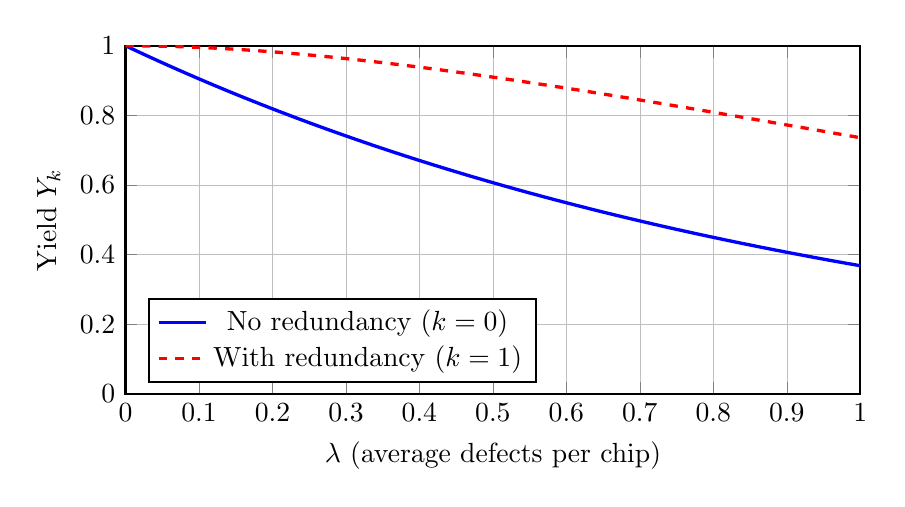
\begin{tikzpicture}
    \begin{axis}[
      width=0.9\linewidth,
      height=6cm,
      xlabel={$\lambda$ (average defects per chip)},
      ylabel={Yield $Y_k$},
      xmin=0, xmax=1,
      ymin=0, ymax=1,
      legend pos=south west,
      grid=both,
      major grid style={line width=.2pt,draw=gray!50},
      minor grid style={line width=.1pt,draw=gray!20},
      thick,
    ]
      \addplot[blue, very thick, domain=0:1, samples=200] {exp(-x)};
      \addlegendentry{No redundancy ($k=0$)}
      \addplot[red, dashed, very thick, domain=0:1, samples=200] {exp(-x)*(1+x)};
      \addlegendentry{With redundancy ($k=1$)}
    \end{axis}
  \end{tikzpicture}
  \caption{Illustrative yield sensitivity (Poisson model) with and without redundancy.}
  \label{fig:yield}
\end{figure}

\section{Educational Application}
\subsection{Teaching Tools}
\begin{itemize}
    \item Cause-effect diagrams: process $\rightarrow$ defect $\rightarrow$ yield
    \item Comparative analysis: 0.25~µm (LOCOS) vs 0.18~µm (STI) for HV devices
    \item Exercises: prioritize process fix vs. redundancy adoption
\end{itemize}

\subsection{Lessons}
This case shows the risk of extrapolating from small macros (500~kbit) to larger ones (1~Mbit) without reassessing defect sensitivity.  
It also emphasizes that process-related instability, invisible at smaller scales, can dominate yield once redundancy is unavailable.  
For embedded SRAM, capacity scaling must always be coupled with explicit yield-risk validation.

\section{Conclusion}
This case demonstrates how HV compatibility constraints dominated node selection.  
Despite the availability of a denser, yield-stable 0.18~µm STI process, the requirement for safe $\sim$30~V HV integration drove adoption of 0.25~µm LOCOS.  
Yield loss from incomplete TiSi\textsubscript{2} phase transformation (with boron absorption) became critical at the 1~Mbit SRAM scale.  
The educational value lies in showing how scaling, process technology, and reliability intersect, and why continuous empirical feedback is essential.

\begin{thebibliography}{99}
\bibitem{Sze2007} S. M. Sze and K. K. Ng, \textit{Physics of Semiconductor Devices}, 3rd ed. Wiley, 2007.
\bibitem{Wolf1986} S. Wolf and R. N. Tauber, \textit{Silicon Processing for the VLSI Era, Vol. 1: Process Technology}. Lattice Press, 1986.
\bibitem{Colinge2004} J.-P. Colinge, \textit{Silicon-on-Insulator Technology: Materials to VLSI}, 3rd ed. Springer, 2004.
\bibitem{ITRS2001} International Technology Roadmap for Semiconductors (ITRS), ``Process Integration, Devices, and Structures,'' 2001.
\bibitem{Takeda1994} E. Takeda, C. Y. Yang, and A. S. Grove, ``Silicide technology for ULSI applications,'' \textit{IEEE Trans. Electron Devices}, vol. 41, no. 12, pp. 2133--2141, Dec. 1994.
\bibitem{Chang1996} J. P. Chang and A. J. Steckl, ``Titanium silicide formation and stability in submicron CMOS technology,'' \textit{J. Appl. Phys.}, vol. 79, no. 9, pp. 4536--4364, 1996.
\end{thebibliography}

\section*{Author Biography}
\textbf{Shinichi Samizo} received the M.S. degree in Electrical and Electronic Engineering from Shinshu University, Japan. 
He worked at Seiko Epson Corporation on semiconductor memory and mixed-signal device development and contributed to inkjet MEMS actuators and PrecisionCore printhead technology. 
He is currently an independent semiconductor researcher focusing on process/device education, memory architecture, and AI system integration.\\
\emph{Contact:} \href{mailto:shin3t72@gmail.com}{shin3t72@gmail.com}\quad
\emph{GitHub:} \href{https://github.com/Samizo-AITL}{Samizo-AITL}.

\end{document}
